\newpage
\chapter{METODE PENELITIAN}
\label{Bab III}

\section{Alur Penelitian}
\label{III.Alur}

Pada penelitian ini, alur dirancang untuk memastikan setiap tahapan pemrosesan dilakukan secara sistematis dan efisien. Alur penelitian ini mencerminkan langkah-langkah utama terkait bagaimana proses yang dilakukan dalam penelitian, dari awal sampai dengan akhir. Gambar dalam bentuk diagram alir (\textit{flowchart}) seperti yang terlihat pada Gambar \ref{fig:3.alur}.

\begin{figure}[H]
\centering
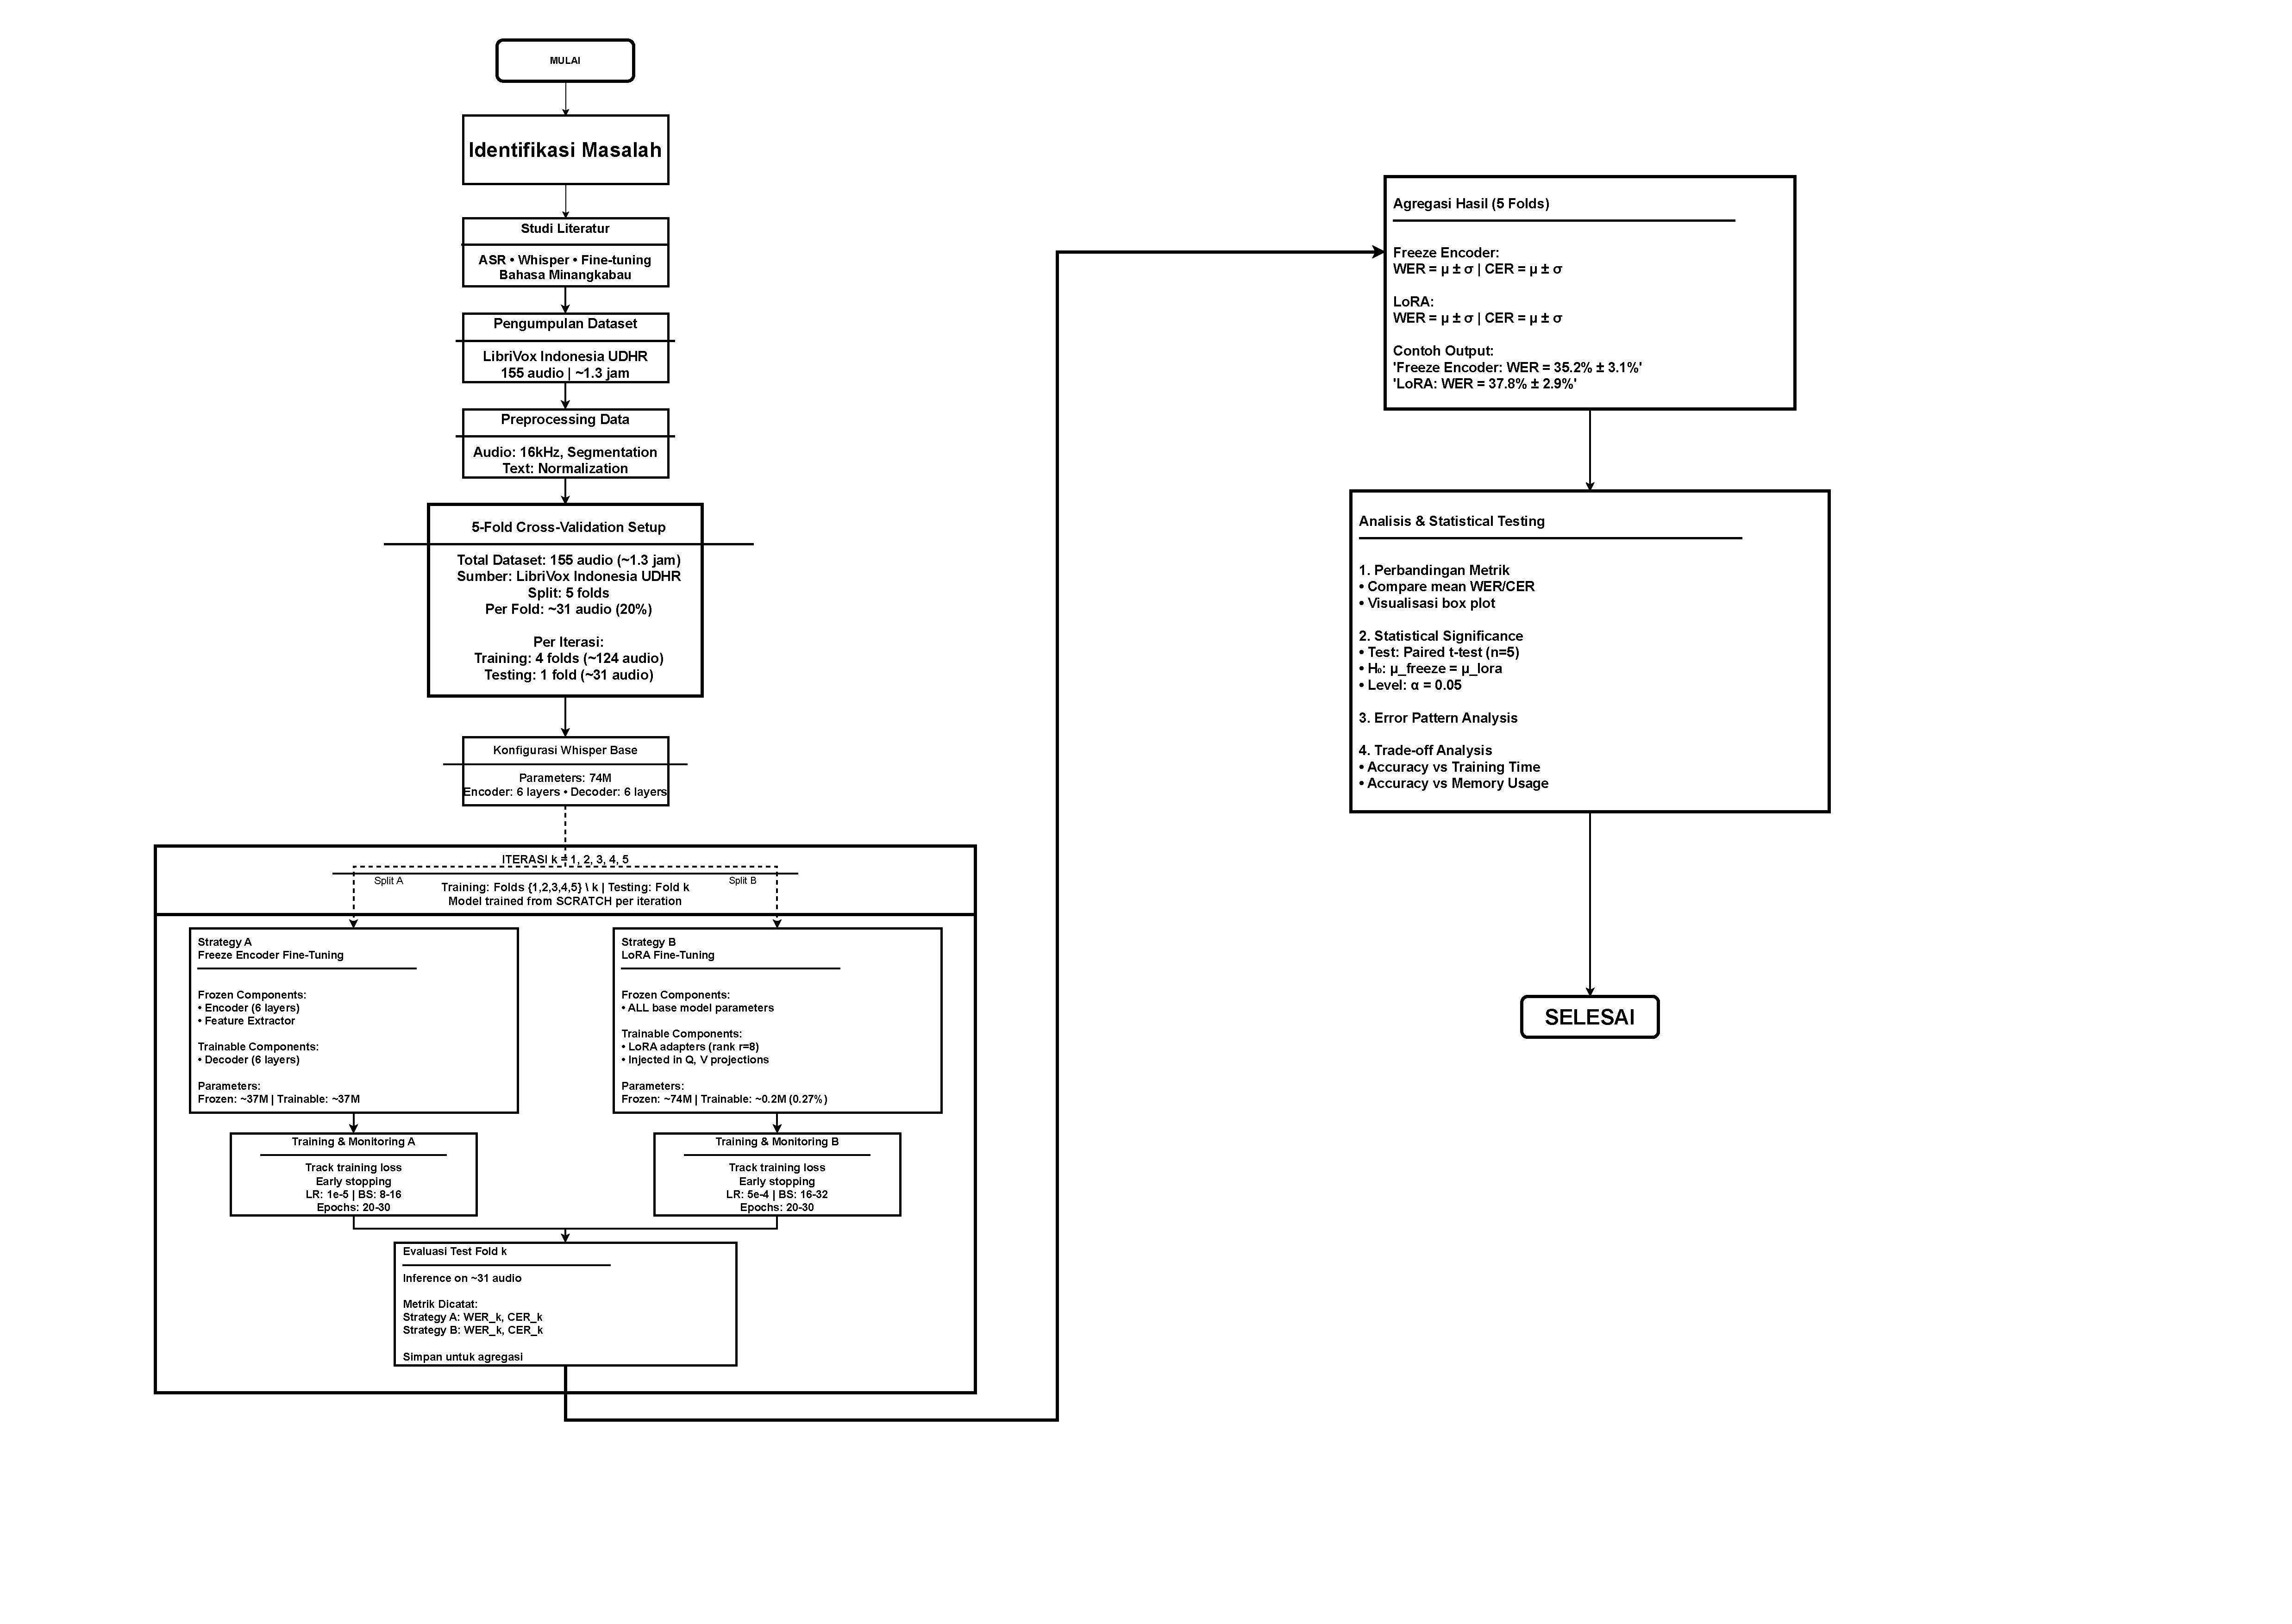
\includegraphics[width=0.6\textwidth]{figure/Alur_Penelitian.pdf}
\caption{Alur Penelitian Fine-Tuning Whisper untuk ASR Bahasa Minangkabau}
\label{fig:3.alur}
\end{figure}

\section{Penjabaran Langkah Penelitian}
\label{III.Jabar Alur}

Penelitian ini dilakukan secara sistematis melalui beberapa tahapan utama yang saling terkait. Setiap tahapan dirancang untuk memastikan model Whisper Small dapat diadaptasi secara optimal untuk mengenali bahasa Minangkabau. Berikut adalah penjabaran detail dari setiap langkah penelitian yang telah digambarkan pada flowchart di Subbab \ref{III.Alur}.

\subsection{Identifikasi Masalah}
\label{III.Langkah1}

Tahap pertama dalam alur penelitian ini adalah identifikasi masalah, yang dilakukan untuk memetakan konteks serta urgensi dari penelitian yang akan dilakukan. Proses ini diawali dengan analisis terhadap permasalahan di dunia nyata, yaitu rendahnya ketersediaan sistem \textit{Automatic Speech Recognition} (ASR) untuk bahasa daerah Indonesia, khususnya bahasa Minangkabau. Analisis ini divalidasi dengan meninjau statistik dan studi terkait yang menunjukkan bahwa sebagian besar sistem ASR komersial yang tersedia saat ini dirancang untuk bahasa-bahasa dengan sumber daya tinggi seperti bahasa Inggris, Mandarin, dan bahasa Eropa lainnya, sementara bahasa daerah Nusantara masih sangat terbatas representasinya.

Setelah urgensi masalah teridentifikasi, proses dilanjutkan dengan menganalisis tantangan spesifik yang dihadapi dalam pengembangan ASR untuk bahasa \textit{low-resource} seperti Minangkabau. Hasil analisis menemukan bahwa tantangan utama terletak pada minimnya ketersediaan dataset audio-transkrip berkualitas tinggi yang diperlukan untuk melatih model ASR. Kondisi ini berbeda dengan bahasa-bahasa besar yang memiliki ribuan jam data audio teranotasi. Identifikasi tantangan \textit{low-resource} ini menegaskan kebutuhan akan pendekatan yang efisien, sehingga penelitian ini difokuskan pada pemanfaatan model \textit{pre-trained} seperti Whisper yang telah dilatih pada skala besar dan dapat diadaptasi untuk bahasa target dengan data yang relatif terbatas.

Berdasarkan analisis tersebut, penelitian ini merumuskan \textit{research gap} yang jelas: belum ada penelitian yang secara komprehensif membandingkan strategi \textit{fine-tuning} yang berbeda (\textit{Full Fine-Tuning} vs LoRA) untuk adaptasi Whisper pada bahasa Minangkabau. Identifikasi masalah ini mencakup beberapa aspek kunci berikut:

\begin{enumerate}[noitemsep]
    \item Analisis keterbatasan sistem ASR \textit{existing} untuk bahasa daerah Indonesia, khususnya dari perspektif ketersediaan model dan dataset
    \item Identifikasi tantangan bahasa \textit{low-resource}: minimnya dataset audio-transkrip Minangkabau yang berkualitas dan teranotasi
    \item Perumusan \textit{research gap}: perlunya adaptasi model \textit{pre-trained} (Whisper) untuk bahasa Minangkabau dengan pendekatan yang efisien secara komputasi
    \item Penetapan objektif penelitian: membandingkan efektivitas strategi \textit{fine-tuning} (\textit{Full Fine-Tuning} vs LoRA) dalam hal akurasi dan efisiensi
    \item Penentuan metrik evaluasi utama: \textit{Word Error Rate} (WER) dan \textit{Character Error Rate} (CER) sebagai indikator kinerja model
\end{enumerate}

\subsection{Studi Literatur}
\label{III.Langkah2}

Setelah masalah utama teridentifikasi, langkah selanjutnya dalam alur penelitian adalah melakukan studi literatur secara sistematis dan komprehensif. Proses ini bertujuan untuk memvalidasi \textit{research gap} yang telah diidentifikasi pada tahap sebelumnya, mengumpulkan landasan teori yang relevan, serta memetakan metode \textit{state-of-the-art} yang akan digunakan sebagai dasar perbandingan dalam penelitian ini. Studi literatur dilakukan dengan pendekatan yang terstruktur untuk memastikan bahwa semua aspek penting dari penelitian tercakup dengan baik.

Studi literatur difokuskan pada empat area utama yang saling berkaitan. Pertama, mendalami arsitektur dan kemampuan model Whisper dari OpenAI, termasuk mekanisme \textit{encoder-decoder Transformer}, proses \textit{pre-training} pada 680,000 jam data multibahasa, dan karakteristik yang membuat Whisper unggul dalam skenario \textit{zero-shot} maupun \textit{few-shot}. Kedua, mengidentifikasi dan menganalisis strategi \textit{fine-tuning} yang telah terbukti efektif untuk bahasa \textit{low-resource}, dengan fokus khusus pada perbandingan antara \textit{Full Fine-Tuning} yang meng-\textit{update} seluruh parameter model versus teknik \textit{Parameter-Efficient Fine-Tuning} (PEFT) seperti LoRA yang hanya melatih sebagian kecil parameter. Ketiga, mempelajari penelitian-penelitian terdahulu yang telah menerapkan Whisper atau model ASR lainnya pada bahasa Indonesia dan bahasa daerah Nusantara, untuk memahami tantangan spesifik dan solusi yang telah dicoba. Keempat, memahami karakteristik linguistik bahasa Minangkabau, termasuk fonologi, morfologi, dan pola ucapan yang dapat mempengaruhi performa model ASR.

Proses studi literatur dilaksanakan melalui tahapan-tahapan berikut:

\begin{enumerate}[noitemsep]
    \item \textit{Review} paper ilmiah terkait Whisper dan strategi \textit{fine-tuning} dari jurnal internasional bereputasi (\textit{e.g.}, ICASSP, Interspeech, ACL) dan \textit{conference proceedings} di bidang \textit{speech processing}
    \item Analisis mendalam terhadap penelitian terdahulu tentang ASR untuk bahasa Indonesia dan bahasa daerah Nusantara, dengan fokus pada metodologi, dataset yang digunakan, dan hasil yang dicapai
    \item Studi dokumentasi teknis OpenAI Whisper dan ekosistem Hugging Face Transformers \textit{library}, termasuk \textit{API reference}, \textit{model cards}, dan \textit{best practices} untuk \textit{fine-tuning}
    \item Eksplorasi metode \textit{fine-tuning} yang tersedia, membandingkan karakteristik \textit{full fine-tuning} dengan pendekatan PEFT seperti LoRA, Adapter, dan Prefix-Tuning
    \item Pemahaman mendalam tentang metrik evaluasi ASR, khususnya \textit{Word Error Rate} (WER) dan \textit{Character Error Rate} (CER), termasuk interpretasi dan keterbatasannya
\end{enumerate}

Hasil dari studi literatur ini menjadi landasan teoritis yang kokoh dalam memilih arsitektur model, menentukan strategi \textit{fine-tuning} yang optimal, dan merancang metodologi evaluasi yang tepat untuk penelitian ini. Selain itu, studi literatur juga mengonfirmasi validitas \textit{research gap} yang telah diidentifikasi dan memberikan justifikasi ilmiah untuk pendekatan yang diusulkan.

\subsection{Pengumpulan Dataset}
\label{III.Langkah3}

Penelitian ini menggunakan dataset publik LibriVox Indonesia versi 1.0, yang merupakan koleksi rekaman audio dari buku-buku domain publik dalam berbagai bahasa daerah Indonesia. Secara spesifik, dataset bahasa Minangkabau yang digunakan berisi rekaman pembacaan \textit{Universal Declaration of Human Rights} (Pernyataan Umum tentang Hak-Hak Asasi Manusia) dalam bahasa Minangkabau. Pemilihan dataset LibriVox Indonesia sebagai sumber data didasarkan pada beberapa pertimbangan penting. Pertama, LibriVox menyediakan audio dengan kualitas rekaman yang relatif baik karena mengikuti standar produksi \textit{audiobook} dengan \textit{sampling rate} 44.1 kHz. Kedua, setiap audio dilengkapi dengan transkrip teks yang akurat karena dibacakan dari naskah tertulis (teks UDHR), sehingga mengurangi beban anotasi manual dan menjamin akurasi transkrip. Ketiga, dataset ini tersedia secara publik dengan lisensi \textit{Public Domain} (CC-0), memungkinkan penggunaan bebas untuk penelitian akademis.

Proses pengumpulan dataset dirancang secara sistematis menggunakan \textit{forced alignment software} yang dikembangkan oleh kontributor LibriVox Indonesia untuk mengkonversi rekaman \textit{audiobook} panjang menjadi segmen-segmen pendek yang sesuai untuk pelatihan ASR. Tahap awal dimulai dengan mengunduh dataset bahasa Minangkabau dari repositori LibriVox Indonesia melalui platform Hugging Face Datasets. Setelah dataset diunduh, dilakukan proses verifikasi kualitas untuk memastikan bahwa setiap segmen audio memiliki kejernihan ucapan yang baik (\textit{clear speech}), minim \textit{background noise}, dan tidak mengandung distorsi audio yang signifikan. Dataset LibriVox Indonesia telah melalui proses segmentasi otomatis yang membagi rekaman panjang menjadi klip-klip pendek dengan durasi beberapa detik hingga maksimal 20 detik, yang ideal untuk pelatihan model ASR.

Dataset bahasa Minangkabau dalam LibriVox Indonesia 1.0 mencakup total sekitar 8 jam rekaman audio dari 7 bahasa Indonesia yang berbeda, dengan porsi spesifik untuk bahasa Minangkabau yang akan digunakan dalam penelitian ini. Meskipun konten terbatas pada pembacaan UDHR, dataset ini tetap mencakup keberagaman \textit{speaker} dengan variasi karakteristik suara yang berbeda. Proses pengumpulan dan persiapan dataset mencakup langkah-langkah berikut:

\begin{enumerate}[noitemsep]
    \item Mengunduh dataset LibriVox Indonesia 1.0 dari Hugging Face Datasets, dengan fokus pada subset bahasa Minangkabau yang berisi pembacaan UDHR
    \item Verifikasi kualitas audio secara teknis untuk setiap segmen: \textit{clear speech}, minimal \textit{background noise}, tidak ada distorsi atau \textit{clipping}
    \item Validasi transkrip teks yang sesuai dengan setiap segmen audio, memastikan akurasi dan kelengkapan transkrip berdasarkan teks UDHR dalam bahasa Minangkabau
    \item Ekstraksi metadata \textit{speaker} (\\textit{reader ID}) untuk analisis keberagaman pembicara dalam dataset
    \item Inventarisasi total durasi audio yang tersedia dan perencanaan penggunaan data untuk mencapai cakupan yang memadai bagi proses \textit{fine-tuning}
\end{enumerate}

Dataset yang berhasil dikumpulkan dari LibriVox Indonesia mencakup rekaman pembacaan UDHR dalam bahasa Minangkabau, yang meskipun terbatas pada satu jenis teks (dokumen deklarasi HAM), tetap merepresentasikan bahasa Minangkabau formal dan standar. Karakteristik dataset ini sesuai untuk penelitian \textit{fine-tuning} model ASR pada bahasa \textit{low-resource}, di mana ketersediaan data yang terbatas merupakan tantangan utama yang perlu diatasi melalui pendekatan \textit{transfer learning} dari model \textit{pre-trained} seperti Whisper.

\subsection{Preprocessing Dataset}
\label{III.Langkah4}

Dataset mentah yang telah dikumpulkan akan melalui tahapan \textit{preprocessing} yang sistematis dan komprehensif untuk memastikan kompatibilitas dengan persyaratan teknis model Whisper serta mengoptimalkan kualitas data yang akan digunakan dalam proses \textit{fine-tuning}. \textit{Preprocessing} merupakan tahap kritis dalam penelitian ini karena kualitas dan konsistensi data input secara langsung mempengaruhi kinerja model ASR yang dilatih. Model Whisper memiliki spesifikasi teknis tertentu, terutama terkait format audio input, yang harus dipenuhi agar model dapat berfungsi secara optimal. Selain itu, \textit{preprocessing} juga bertujuan untuk standardisasi data sehingga mengurangi variabilitas yang tidak relevan dan memungkinkan model fokus pada pembelajaran pola linguistik yang penting.

Proses \textit{preprocessing} dirancang dalam tiga tahap utama yang saling melengkapi: \textit{audio preprocessing}, \textit{text preprocessing}, dan \textit{dataset splitting}. Setiap tahap memiliki tujuan spesifik dan menggunakan teknik-teknik yang telah terbukti efektif dalam penelitian ASR sebelumnya. Pendekatan sistematis ini memastikan bahwa dataset yang dihasilkan memiliki kualitas yang konsisten, kompatibel dengan arsitektur Whisper, dan siap digunakan untuk proses \textit{training}, \textit{validation}, dan \textit{testing}.

\subsubsection{Audio Preprocessing}

Tahap \textit{audio preprocessing} berfokus pada transformasi sinyal audio mentah menjadi format yang sesuai dengan spesifikasi teknis Whisper dan mengoptimalkan kualitas sinyal untuk pembelajaran model. Proses ini mencakup beberapa operasi penting:

\begin{enumerate}[noitemsep]
    \item \textbf{Format Conversion}: Konversi format audio dari MP3 (format asli LibriVox Indonesia) ke WAV (\textit{Waveform Audio File Format}). Konversi ini diperlukan karena format MP3 yang terkompresi dengan \textit{lossy compression} memerlukan proses \textit{decoding} tambahan yang dapat membebani komputasi Whisper. Format WAV yang \textit{uncompressed} memungkinkan akses langsung ke data audio mentah (\textit{raw audio samples}), sehingga mengurangi beban komputasi dan mempercepat proses \textit{preprocessing} serta \textit{training}
    \item \textbf{Resampling}: Konversi \textit{sampling rate} audio dari 44.1 kHz (format asli LibriVox Indonesia) ke 16 kHz, yang merupakan spesifikasi standar yang digunakan oleh model Whisper. Konversi ini penting karena model Whisper dilatih dengan data audio pada frekuensi 16 kHz dan akan menghasilkan performa optimal pada \textit{sampling rate} yang sama
    \item \textbf{Segmentation}: Pemotongan audio panjang menjadi \textit{clips} dengan durasi 10-30 detik untuk meningkatkan efisiensi \textit{training} dan mengurangi penggunaan memori GPU. Segmentasi juga membantu model mempelajari pola dalam konteks yang lebih terfokus
    \item \textbf{Normalization}: Normalisasi \textit{amplitude} audio untuk memastikan konsistensi volume di seluruh dataset, menghindari bias model terhadap audio dengan volume tertentu
    \item \textbf{Silence Removal}: Penghapusan periode \textit{silence} yang tidak informatif di awal dan akhir setiap \textit{clip}, sehingga model tidak perlu memproses bagian audio yang tidak mengandung informasi linguistik
    \item \textbf{Quality Check}: Penyaringan \textit{clips} dengan \textit{Signal-to-Noise Ratio} (SNR) rendah atau mengandung distorsi signifikan, untuk memastikan hanya data berkualitas tinggi yang digunakan dalam \textit{training}
\end{enumerate}

\subsubsection{Text Preprocessing}

Tahap \textit{text preprocessing} bertujuan untuk menstandarkan transkrip teks dan menghilangkan variasi yang tidak relevan untuk tugas ASR. Standarisasi teks penting untuk memastikan konsistensi dalam pelatihan model dan evaluasi hasil. Proses ini mencakup:

\begin{enumerate}[noitemsep]
    \item \textbf{Lowercase Conversion}: Konversi semua teks ke huruf kecil untuk mengurangi ukuran \textit{vocabulary} dan menghilangkan perbedaan yang tidak relevan antara kapitalisasi
    \item \textbf{Punctuation Normalization}: Standarisasi tanda baca untuk konsistensi format, termasuk normalisasi tanda kutip, tanda hubung, dan simbol-simbol khusus
    \item \textbf{Number Normalization}: Konversi representasi numerik menjadi bentuk kata (\textit{e.g.}, "10" $\rightarrow$ "sepuluh", "2025" $\rightarrow$ "dua ribu dua puluh lima") untuk konsistensi dengan bagaimana angka diucapkan dalam bahasa Minangkabau
    \item \textbf{Whitespace Normalization}: Pembersihan spasi berlebih, tab, dan karakter \textit{whitespace} lainnya untuk memastikan format teks yang konsisten
    \item \textbf{Special Character Handling}: Penanganan khusus untuk karakter-karakter yang spesifik dalam bahasa Minangkabau, termasuk diakritik atau simbol yang mungkin muncul dalam transkrip
\end{enumerate}

\subsubsection{Dataset Splitting}

Setelah \textit{preprocessing} audio dan teks selesai, dataset dibagi menjadi tiga subset dengan proporsi yang standar dalam penelitian \textit{machine learning}:

\begin{itemize}[noitemsep]
    \item \textit{Training set}: 80\% dari total data, digunakan untuk melatih parameter model
    \item \textit{Validation set}: 10\% dari total data, digunakan untuk memantau performa selama \textit{training} dan melakukan \textit{hyperparameter tuning}
    \item \textit{Test set}: 10\% dari total data, digunakan untuk evaluasi final dan tidak pernah dilihat oleh model selama \textit{training}
\end{itemize}

Pembagian dilakukan secara \textit{stratified} untuk memastikan distribusi \textit{speaker}, dialek Minangkabau, dan karakteristik lainnya seimbang di setiap subset. Pendekatan \textit{stratified splitting} ini penting untuk menghindari bias dalam evaluasi dan memastikan bahwa setiap subset merepresentasikan keberagaman yang ada dalam dataset lengkap.

\subsection{Konfigurasi Model Whisper Small}
\label{III.Langkah5}

Model Whisper Small dipilih sebagai arsitektur \textit{base model} dalam penelitian ini berdasarkan pertimbangan yang cermat terhadap \textit{trade-off} antara performa, efisiensi komputasi, dan kelayakan untuk skenario \textit{low-resource}. Whisper Small, dengan 244 juta parameter, merupakan varian menengah dari keluarga model Whisper yang menawarkan keseimbangan optimal: cukup besar untuk menangkap kompleksitas bahasa tetapi tidak terlalu besar sehingga memerlukan sumber daya komputasi yang tidak realistis untuk \textit{fine-tuning} pada infrastruktur \textit{cloud} yang tersedia seperti RunPod. Pemilihan ini juga didukung oleh studi-studi sebelumnya yang menunjukkan bahwa Whisper Small dapat mencapai performa yang kompetitif pada berbagai tugas ASR, terutama setelah di-\textit{fine-tune} pada bahasa target.

Arsitektur Whisper Small menggunakan \textit{encoder-decoder Transformer} dengan konfigurasi yang telah dioptimalkan untuk tugas \textit{speech recognition}. Model ini telah di-\textit{pre-train} pada dataset multibahasa yang sangat besar (680,000 jam audio) sehingga memiliki representasi yang kuat tentang pola akustik dan linguistik lintas bahasa. Karakteristik \textit{pre-trained} ini memungkinkan model untuk di-\textit{transfer} dengan efisien ke bahasa Minangkabau meskipun dengan data \textit{fine-tuning} yang relatif terbatas (10-20 jam). Proses konfigurasi model dilakukan secara sistematis untuk memastikan semua komponen berfungsi dengan benar dan siap untuk tahap \textit{fine-tuning}.

Tahap konfigurasi model Whisper Small mencakup beberapa langkah teknis penting:

\begin{enumerate}[noitemsep]
    \item \textit{Loading pre-trained} Whisper Small (244M \textit{parameters}) dari Hugging Face Model Hub menggunakan \textit{library} Transformers, memastikan model dalam keadaan \textit{pre-trained} yang telah terbukti efektif
    \item Verifikasi arsitektur model: 12 \textit{encoder layers} dan 12 \textit{decoder layers}, dengan \textit{hidden dimension} (\textit{width}) 768 dan 12 \textit{attention heads} per \textit{layer}, sesuai dengan spesifikasi resmi Whisper Small
    \item Inisialisasi \textit{tokenizer} dengan \textit{vocabulary} sebesar 51,864 \textit{tokens}, yang mencakup representasi karakter dan subword untuk berbagai bahasa termasuk kemampuan untuk mengakomodasi bahasa baru
    \item Konfigurasi \textit{feature extractor} untuk menghasilkan representasi \textit{log-Mel spectrogram} dengan 80 dimensi, menggunakan \textit{window size} 25ms dan \textit{hop length} 10ms, yang merupakan parameter standar untuk ekstraksi fitur audio dalam Whisper
    \item \textit{Setup device} (GPU/CPU) untuk \textit{training}, dengan preferensi GPU (NVIDIA GeForce RTX 4090 dengan 24 GB VRAM) untuk mempercepat komputasi matriks dalam proses \textit{fine-tuning}
\end{enumerate}

\subsection{Implementasi Fine-Tuning}
\label{III.Langkah6}

Penelitian ini menerapkan pendekatan komparatif dengan membandingkan dua strategi \textit{fine-tuning} yang berbeda: \textit{Full Fine-Tuning} dan \textit{Low-Rank Adaptation} (LoRA). Pemilihan kedua strategi ini didasarkan pada karakteristik yang saling melengkapi dalam konteks bahasa \textit{low-resource}. \textit{Full Fine-Tuning} merepresentasikan pendekatan tradisional yang meng-\textit{update} seluruh parameter model, berpotensi menghasilkan adaptasi yang paling optimal tetapi dengan biaya komputasi yang tinggi. Sebaliknya, LoRA merupakan teknik \textit{Parameter-Efficient Fine-Tuning} (PEFT) yang hanya melatih sebagian kecil parameter tambahan, menawarkan efisiensi komputasi yang signifikan dengan trade-off minimal dalam akurasi. Implementasi kedua metode dilakukan secara terpisah dan sistematis untuk memastikan perbandingan yang adil dan valid.

Pendekatan komparatif ini memungkinkan analisis mendalam terhadap \textit{trade-off} antara akurasi model dan efisiensi sumber daya. Dalam konteks bahasa Minangkabau sebagai bahasa \textit{low-resource}, pertanyaan penting yang perlu dijawab adalah: apakah efisiensi LoRA (dengan hanya melatih $\sim$2\% parameter) memberikan hasil yang sebanding dengan \textit{Full Fine-Tuning} (yang melatih 100\% parameter)? Jika LoRA dapat mencapai performa yang mendekati \textit{Full Fine-Tuning} dengan biaya komputasi yang jauh lebih rendah, maka LoRA menjadi solusi yang lebih praktis dan dapat diskalakan untuk bahasa-bahasa \textit{low-resource} lainnya. Untuk menjawab pertanyaan ini, implementasi kedua metode dirancang dengan cermat dengan pengaturan \textit{hyperparameter} yang dioptimalkan untuk masing-masing pendekatan.

\subsubsection{Full Fine-Tuning}

Pada metode \textit{Full Fine-Tuning}, seluruh 244 juta parameter model Whisper Small di-\textit{update} selama proses \textit{training}. Pendekatan ini memberikan fleksibilitas maksimal bagi model untuk beradaptasi dengan karakteristik spesifik bahasa Minangkabau, termasuk pola fonetik, intonasi, dan struktur linguistik yang unik. Konfigurasi \textit{training} untuk \textit{Full Fine-Tuning} adalah sebagai berikut:

\begin{enumerate}[noitemsep]
    \item \textbf{Optimizer}: AdamW (\textit{Adam with Weight Decay}) dengan \textit{weight decay} 0.01 untuk regularisasi dan mencegah \textit{overfitting}
    \item \textbf{Learning Rate}: $2 \times 10^{-5}$ dengan strategi \textit{linear warmup} (500 langkah) diikuti \textit{cosine decay} untuk konvergensi yang stabil
    \item \textbf{Batch Size}: 16 sampel per \textit{batch}, dengan opsi \textit{gradient accumulation} jika memori GPU tidak mencukupi
    \item \textbf{Epochs}: 10-15 \textit{epochs} dengan mekanisme \textit{early stopping} (\textit{patience}=5) untuk menghentikan \textit{training} jika tidak ada peningkatan pada \textit{validation} WER
    \item \textbf{Loss Function}: \textit{Cross-entropy loss} standar untuk tugas klasifikasi sekuens
\end{enumerate}

\subsubsection{LoRA Fine-Tuning}

Metode LoRA (\textit{Low-Rank Adaptation}) bekerja dengan menambahkan matriks \textit{low-rank} sebagai parameter yang dapat dilatih pada \textit{attention layers}, sementara seluruh parameter \textit{pre-trained} dari Whisper Small tetap \textit{frozen}. Pendekatan ini sangat efisien karena hanya melatih $\sim$2\% dari total parameter (sekitar 5 juta parameter dari 244 juta), namun tetap mampu mencapai performa yang kompetitif. Konfigurasi LoRA \textit{fine-tuning} adalah sebagai berikut:

\begin{enumerate}[noitemsep]
    \item \textbf{LoRA Configuration}:
    \begin{itemize}[noitemsep]
        \item \textit{Rank} ($r$): 8 (dimensi matriks \textit{low-rank} yang ditambahkan)
        \item \textit{Alpha}: 16 (\textit{scaling factor} untuk LoRA \textit{updates})
        \item \textit{Dropout}: 0.1 (regularisasi pada LoRA \textit{layers})
        \item \textit{Target modules}: \textit{Query} dan \textit{Value projections} dalam \textit{attention layers}, yang merupakan komponen paling kritis untuk adaptasi
    \end{itemize}
    \item \textbf{Trainable Parameters}: $\sim$2\% dari total parameter ($\sim$5 juta parameter), drastis lebih sedikit dibanding \textit{Full Fine-Tuning}
    \item \textbf{Optimizer}: AdamW dengan \textit{weight decay} 0.01
    \item \textbf{Learning Rate}: $5 \times 10^{-4}$ (lebih tinggi dibanding \textit{Full FT} karena hanya melatih sebagian kecil parameter pada \textit{frozen base model})
    \item \textbf{Batch Size}: 16 sampel per \textit{batch}
    \item \textbf{Epochs}: 10-15 \textit{epochs} dengan \textit{early stopping} (\textit{patience}=5)
\end{enumerate}

\subsubsection{Data Augmentation}

Untuk meningkatkan \textit{robustness} model pada skenario \textit{low-resource} dan mencegah \textit{overfitting} pada dataset yang relatif kecil, diterapkan beberapa teknik \textit{data augmentation} pada data audio selama \textit{training}:

\begin{enumerate}[noitemsep]
    \item \textbf{SpecAugment}: Teknik \textit{augmentation} pada representasi spektrogram dengan menerapkan \textit{time masking} (T=70) dan \textit{frequency masking} (F=27) untuk meningkatkan invariansi temporal dan frekuensi
    \item \textbf{Speed Perturbation}: Variasi kecepatan audio dengan faktor $\{0.9, 1.0, 1.1\}$ untuk mensimulasikan variasi kecepatan bicara alami
    \item \textbf{Noise Injection}: Penambahan \textit{environmental noise} dengan SNR 15-25 dB untuk meningkatkan \textit{robustness} model terhadap kondisi audio yang beragam
\end{enumerate}

\subsubsection{Regularization}

Selain \textit{data augmentation}, beberapa teknik \textit{regularization} juga diterapkan untuk mencegah \textit{overfitting} dan meningkatkan generalisasi model:

\begin{enumerate}[noitemsep]
    \item \textit{Dropout} pada \textit{attention layers} (p=0.1) dan \textit{feed-forward network} (FFN) \textit{layers} (p=0.3) untuk mengurangi \textit{co-adaptation} antar \textit{neurons}
    \item \textit{Label smoothing} ($\epsilon = 0.1$) untuk mencegah overconfidence pada prediksi dan meningkatkan kalibrasi model
    \item \textit{Gradient clipping} (\textit{max norm} = 1.0) untuk mencegah \textit{exploding gradients} selama \textit{training}
    \item \textit{Early stopping} berdasarkan \textit{validation} WER, menghentikan \textit{training} jika tidak ada perbaikan selama 5 \textit{epochs} berturut-turut
\end{enumerate}

\subsection{Training dan Monitoring}
\label{III.Langkah7}

Proses \textit{training} dilakukan dengan protokol \textit{monitoring} yang ketat dan sistematis untuk memastikan konvergensi yang optimal serta mendeteksi potensi masalah sejak dini. \textit{Monitoring} yang komprehensif sangat penting dalam penelitian ini mengingat kompleksitas model Whisper dan sifat dataset yang \textit{low-resource}. Tanpa \textit{monitoring} yang tepat, berbagai masalah seperti \textit{overfitting}, konvergensi yang lambat, atau konfigurasi \textit{hyperparameter} yang tidak optimal dapat tidak terdeteksi dan menghasilkan model dengan performa suboptimal. Oleh karena itu, strategi \textit{monitoring} dirancang untuk memberikan visibilitas penuh terhadap seluruh aspek proses \textit{training}, dari metrik performa hingga penggunaan sumber daya komputasi.

Infrastruktur \textit{training} menggunakan RunPod \textit{Cloud GPU Service} dengan NVIDIA GeForce RTX 4090 (24 GB VRAM), yang menyediakan performa komputasi tinggi untuk \textit{fine-tuning} model berukuran menengah seperti Whisper Small. Seluruh proses \textit{training} untuk kedua strategi (\textit{Full Fine-Tuning} dan LoRA) dilakukan pada infrastruktur yang sama untuk memastikan perbandingan yang adil. Metrik-metrik kunci dicatat secara otomatis menggunakan \textit{logging framework} yang terintegrasi, dan \textit{checkpointing} dilakukan secara berkala untuk menyimpan \textit{state} model terbaik.

Protokol \textit{training} dan \textit{monitoring} yang diterapkan mencakup aspek-aspek berikut:

\begin{enumerate}[noitemsep]
    \item \textit{Training} dilakukan pada RunPod dengan akselerasi GPU NVIDIA GeForce RTX 4090 (24 GB VRAM) untuk mempercepat komputasi matriks dalam \textit{backpropagation}
    \item \textit{Logging} metrik setiap 100 \textit{steps}: \textit{training loss}, \textit{learning rate} saat ini, dan waktu komputasi per \textit{batch}, untuk memantau progres \textit{training} secara real-time
    \item Evaluasi pada \textit{validation set} setiap \textit{epoch}: perhitungan WER, CER, dan \textit{validation loss} untuk memantau kemampuan generalisasi model
    \item \textit{Checkpoint} model terbaik berdasarkan \textit{lowest validation} WER, memastikan model yang disimpan adalah yang paling optimal untuk tugas ASR bahasa Minangkabau
    \item \textit{Tracking training time} dan penggunaan memori GPU untuk analisis efisiensi komputasi, terutama penting untuk membandingkan \textit{Full Fine-Tuning} dengan LoRA
    \item Visualisasi \textit{learning curves} (\textit{loss}, WER, CER vs \textit{epochs}) menggunakan \textit{TensorBoard} atau \textit{Weights \& Biases} untuk analisis visual terhadap konvergensi model
\end{enumerate}

\subsection{Evaluasi Model}
\label{III.Langkah8}

Model yang telah di-\textit{fine-tune} dievaluasi secara komprehensif menggunakan \textit{test set} yang tidak pernah dilihat oleh model selama proses \textit{training} maupun \textit{validation}. Prinsip isolasi \textit{test set} ini sangat penting untuk memastikan bahwa metrik evaluasi yang diperoleh merepresentasikan kemampuan generalisasi model yang sebenarnya pada data baru, bukan hanya kemampuan menghafal pola dalam data \textit{training}. Evaluasi dilakukan dengan protokol yang konsisten untuk kedua strategi \textit{fine-tuning} (\textit{Full Fine-Tuning} dan LoRA) untuk memungkinkan perbandingan yang adil dan valid.

Proses evaluasi dirancang untuk mengukur berbagai aspek performa model, tidak hanya akurasi transkrip tetapi juga \textit{error patterns} dan karakteristik kesalahan yang terjadi. Analisis \textit{error patterns} memberikan \textit{insights} penting tentang jenis kesalahan yang paling sering dibuat model (substitusi, penghapusan, atau penyisipan kata), yang dapat menjadi dasar untuk perbaikan model di masa depan. Selain itu, evaluasi juga mempertimbangkan variasi dialek Minangkabau jika memungkinkan, untuk memahami seberapa baik model dapat menangani keberagaman linguistik dalam bahasa target.

Protokol evaluasi yang diterapkan mencakup tahapan-tahapan berikut:

\begin{enumerate}[noitemsep]
    \item \textit{Inference} pada \textit{test set} menggunakan algoritma \textit{beam search} dengan \textit{beam size} = 5, yang memberikan keseimbangan antara kualitas transkrip dan kecepatan inferensi
    \item Perhitungan \textit{Word Error Rate} (WER) sebagai metrik utama untuk mengukur akurasi transkrip pada level kata
    \item Perhitungan \textit{Character Error Rate} (CER) sebagai metrik tambahan yang lebih sensitif terhadap kesalahan fonetik dan memberikan perspektif komplementer terhadap WER
    \item Normalisasi teks sebelum evaluasi (konversi ke \textit{lowercase}, penghapusan tanda baca, normalisasi\textit{whitespace}) untuk memastikan konsistensi dalam perhitungan metrik
    \item Analisis \textit{error patterns} detail dengan mengkategorikan kesalahan menjadi: substitusi (kata yang salah diganti), penghapusan (kata yang hilang), dan penyisipan (kata tambahan yang tidak seharusnya ada)
    \item Perbandingan performa antara model \textit{Full Fine-Tuning} dan LoRA menggunakan metrik WER, CER, serta analisis \textit{trade-off} dengan waktu \textit{training} dan penggunaan memori
    \item Evaluasi per-dialek Minangkabau (\textit{e.g.}, dialek Padang, Bukittinggi, Payakumbuh) jika distribusi data memungkinkan, untuk memahami kemampuan model menangani variasi linguistik
\end{enumerate}

\subsection{Analisis Hasil dan Perbandingan}
\label{III.Langkah9}

Tahap akhir dari alur penelitian adalah melakukan analisis mendalam terhadap hasil evaluasi dan membandingkan performa antara dua strategi \textit{fine-tuning} yang telah diimplementasikan. Analisis ini tidak hanya berfokus pada perbandingan metrik akurasi (WER dan CER), tetapi juga mempertimbangkan aspek-aspek praktis lainnya seperti efisiensi komputasi, waktu \textit{training}, penggunaan memori, dan kelayakan untuk deployment. Pendekatan analisis komparatif ini bertujuan untuk memberikan rekomendasi yang komprehensif dan berbasis bukti mengenai strategi \textit{fine-tuning} yang paling sesuai untuk adaptasi Whisper pada bahasa Minangkabau dan bahasa \textit{low-resource} lainnya.

Analisis dilakukan dengan mengintegrasikan evaluasi kuantitatif (metrik numerik) dan kualitatif (analisis transkrip), memberikan pemahaman yang holistik tentang kekuatan dan kelemahan masing-masing strategi. Evaluasi kuantitatif mencakup perbandingan statistik WER dan CER, sementara evaluasi kualitatif melibatkan inspeksi manual terhadap sampel transkrip untuk mengidentifikasi pola kesalahan yang mungkin tidak tertangkap oleh metrik numerik. Pendekatan ganda ini memastikan bahwa kesimpulan yang ditarik tidak hanya berdasarkan angka-angka tetapi juga didukung oleh pemahaman mendalam tentang perilaku model.

Proses analisis hasil dan perbandingan mencakup aspek-aspek berikut:

\begin{enumerate}[noitemsep]
    \item Perbandingan metrik WER dan CER antara \textit{Full Fine-Tuning} dan LoRA pada \textit{test set} yang sama, termasuk perhitungan selisih performa dan signifikansi statistik perbedaan tersebut
    \item Analisis \textit{trade-off} multidimensional: akurasi model vs efisiensi \textit{training} (waktu pelatihan, penggunaan memori GPU, jumlah parameter yang dilatih), untuk mengidentifikasi strategi yang menawarkan keseimbangan terbaik
    \item Evaluasi kualitas transkrip secara kualitatif melalui inspeksi manual terhadap sampel transkrip, mengidentifikasi jenis kesalahan yang paling umum dan konteks di mana setiap metode unggul atau lemah
    \item Identifikasi \textit{patterns of errors} yang spesifik (\textit{common misrecognitions}), seperti fonem atau kata Minangkabau yang sering salah dikenali, untuk memberikan \textit{insights} bagi penelitian lanjutan
    \item Analisis performa pada \textit{different speaking styles} (\textit{e.g.}, narasi formal vs informal) dan dialek Minangkabau yang berbeda, jika distribusi data memungkinkan
    \item Diskusi tentang \textit{limitations} penelitian (\textit{e.g.}, ukuran dataset yang terbatas, variasi dialek yang tidak sepenuhnya tercakup) dan \textit{potential improvements} untuk penelitian masa depan
    \item Perumusan rekomendasi strategi \textit{fine-tuning} terbaik untuk bahasa Minangkabau berdasarkan hasil analisis komprehensif, dengan pertimbangan terhadap konteks penggunaan (\textit{e.g.}, penelitian akademis vs aplikasi praktis)
\end{enumerate}

\section{Alat dan Bahan Tugas Akhir}
\label{III.Alat dan Bahan}

Penelitian ini memerlukan berbagai alat dan bahan untuk mendukung implementasi dan evaluasi model ASR bahasa Minangkabau.

\subsection{Alat}
\label{III.Alat}

Alat-alat yang digunakan dalam penelitian ini meliputi perangkat keras dan perangkat lunak:

\subsubsection{Perangkat Keras}

\begin{enumerate}[noitemsep]
    \item \textbf{Laptop}: ASUS VivoBook 14 K413 (11th Gen Intel), digunakan untuk \textit{development}, analisis data, dan penulisan kode
    \begin{itemize}[noitemsep]
        \item Processor: Intel Core i3 (11th Generation)
        \item RAM: 8 GB DDR4
        \item Storage: 512 GB SSD
        \item Sistem operasi: Linux/Windows
        \item Fungsi: \textit{Development environment}, eksplorasi data, dan analisis hasil
    \end{itemize}
    \item \textbf{RunPod Cloud GPU Service}: Platform \textit{cloud computing} untuk \textit{training} model dengan GPU
    \begin{itemize}[noitemsep]
        \item GPU: NVIDIA GeForce RTX 4090 (24 GB VRAM)
        \item RAM: 36 GB
        \item vCPU: 8 \textit{virtual cores}
        \item Storage: 80 GB \textit{disk space}
        \item Container: \texttt{runpod/pytorch:1.0.2-cu1281-torch280-ubuntu2404}
        \item Fungsi: \textit{Training} model \textit{Full Fine-Tuning} dan LoRA dengan akselerasi GPU
    \end{itemize}
\end{enumerate}

\subsubsection{Perangkat Lunak}

\begin{enumerate}[noitemsep]
    \item \textbf{Python 3.10+}: Bahasa pemrograman utama untuk implementasi model dan \textit{data processing}
    \item \textbf{PyTorch 2.8.0}: \textit{Deep learning framework} untuk \textit{training} dan \textit{inference} model Whisper
    \item \textbf{CUDA 12.8.1}: \textit{NVIDIA CUDA Toolkit} untuk akselerasi GPU pada RunPod
    \item \textbf{Ubuntu 24.04 LTS}: Sistem operasi \textit{Linux} pada \textit{container} RunPod (\texttt{runpod/pytorch:1.0.2-cu1281-torch280-ubuntu2404})
    \item \textbf{Hugging Face Transformers}: \textit{Library} untuk memuat dan \textit{fine-tune} model Whisper \textit{pre-trained}
    \item \textbf{Hugging Face Datasets}: \textit{Library} untuk manajemen dataset, \textit{data loading}, dan \textit{streaming} dari Hugging Face Hub
    \item \textbf{Hugging Face Accelerate}: \textit{Library} untuk \textit{distributed training}, optimisasi memori, dan akselerasi proses \textit{training} pada GPU
    \item \textbf{Hugging Face Evaluate}: \textit{Library} untuk evaluasi metrik model \textit{machine learning} secara standar dan konsisten
    \item \textbf{PEFT (Parameter-Efficient Fine-Tuning)}: \textit{Library} dari Hugging Face untuk implementasi LoRA dan metode \textit{fine-tuning} yang efisien parameter
    \item \textbf{torchaudio}: \textit{Library} PyTorch untuk \textit{audio processing}, transformasi, dan augmentasi data audio
    \item \textbf{torchcodec}: \textit{Library} untuk \textit{encoding} dan \textit{decoding} berbagai format audio dengan \textit{backend} PyTorch
    \item \textbf{audiomentations}: \textit{Library} untuk \textit{data augmentation} audio (\textit{noise injection}, \textit{pitch shifting}, \textit{time stretching})
    \item \textbf{jiwer}: \textit{Library} untuk perhitungan metrik evaluasi ASR (WER dan CER)
    \item \textbf{scikit-learn}: \textit{Library} untuk utilitas \textit{machine learning} (\textit{data splitting}, metrik evaluasi, \textit{preprocessing})
    \item \textbf{TensorBoard}: Platform visualisasi untuk \textit{monitoring} metrik \textit{training}, \textit{loss curves}, dan parameter model secara \textit{real-time}
    \item \textbf{Weights \& Biases (wandb)}: Platform untuk \textit{experiment tracking}, visualisasi \textit{learning curves}, perbandingan eksperimen, dan \textit{logging} metrik
    \item \textbf{Jupyter Notebook}: \textit{Interactive development environment} untuk eksplorasi data, eksperimen model, dan dokumentasi proses penelitian
    \item \textbf{Git/GitHub}: \textit{Version control system} dan repositori kode untuk manajemen proyek dan kolaborasi
    \item \textbf{Visual Studio Code}: \textit{Code editor} untuk \textit{local development} pada ASUS VivoBook 14 K413
\end{enumerate}

\subsection{Bahan}
\label{III.Bahan}

Bahan-bahan yang digunakan dalam penelitian ini meliputi dataset dan dokumen referensi:

\begin{enumerate}[noitemsep]
    \item \textbf{Dataset Audio Bahasa Minangkabau}:
    \begin{itemize}[noitemsep]
        \item Sumber: LibriVox Indonesia 1.0 via Hugging Face Datasets (\url{https://huggingface.co/datasets/indonesian-nlp/librivox-indonesia})
        \item Konten: Pembacaan \textit{Universal Declaration of Human Rights} dalam bahasa Minangkabau
        \item Format: Audio \textit{files} MP3 dengan \textit{sampling rate} 44.1 kHz
        \item Durasi: Sekitar 8 jam total (7 bahasa), subset Minangkabau digunakan untuk penelitian
        \item Segmentasi: Klip audio dengan durasi beberapa detik hingga maksimal 20 detik
        \item Lisensi: \textit{Public Domain} (CC-0)
    \end{itemize}
    \item \textbf{Model Pre-trained}:
    \begin{itemize}[noitemsep]
        \item Whisper Small dari OpenAI (via Hugging Face Model Hub)
        \item Model ID: \texttt{openai/whisper-small}
        \item Lisensi: MIT License
    \end{itemize}
    \item \textbf{Dokumen Referensi}:
    \begin{itemize}[noitemsep]
        \item Paper: "Robust Speech Recognition via Large-Scale Weak Supervision" \cite{radford2023whisper}
        \item Paper: "LoRA: Low-Rank Adaptation of Large Language Models" \cite{hu2022lora}
        \item Paper: "Exploration of Whisper Fine-Tuning Strategies for Low-Resource ASR" \cite{liu2024exploration}
        \item Dokumentasi Hugging Face Transformers
        \item Dokumentasi PEFT library
    \end{itemize}
\end{enumerate}

\section{Metode Pengembangan}
\label{III.Metode}

Penelitian ini menggunakan pendekatan eksperimental dengan metodologi yang terstruktur untuk memastikan validitas dan reproducibility hasil.

\subsection{Pendekatan Penelitian}
\label{III.Pendekatan}

Penelitian ini mengadopsi \textbf{pendekatan eksperimental} dengan karakteristik:

\begin{enumerate}[noitemsep]
    \item \textbf{Quantitative Evaluation}: Pengukuran performa menggunakan metrik objektif (WER, CER)
    \item \textbf{Comparative Study}: Perbandingan antara dua strategi fine-tuning (Full vs LoRA)
    \item \textbf{Controlled Experiment}: Dataset, hyperparameters, dan evaluation protocol dijaga konsisten
    \item \textbf{Reproducible Research}: Semua kode, konfigurasi, dan hasil didokumentasikan
\end{enumerate}

\subsection{Alur Pengembangan}
\label{III.Alur_Pengembangan}

Pengembangan sistem ASR bahasa Minangkabau mengikuti alur yang sistematis seperti digambarkan pada Gambar \ref{fig:3.alur_dev}:

\begin{figure}[H]
\centering
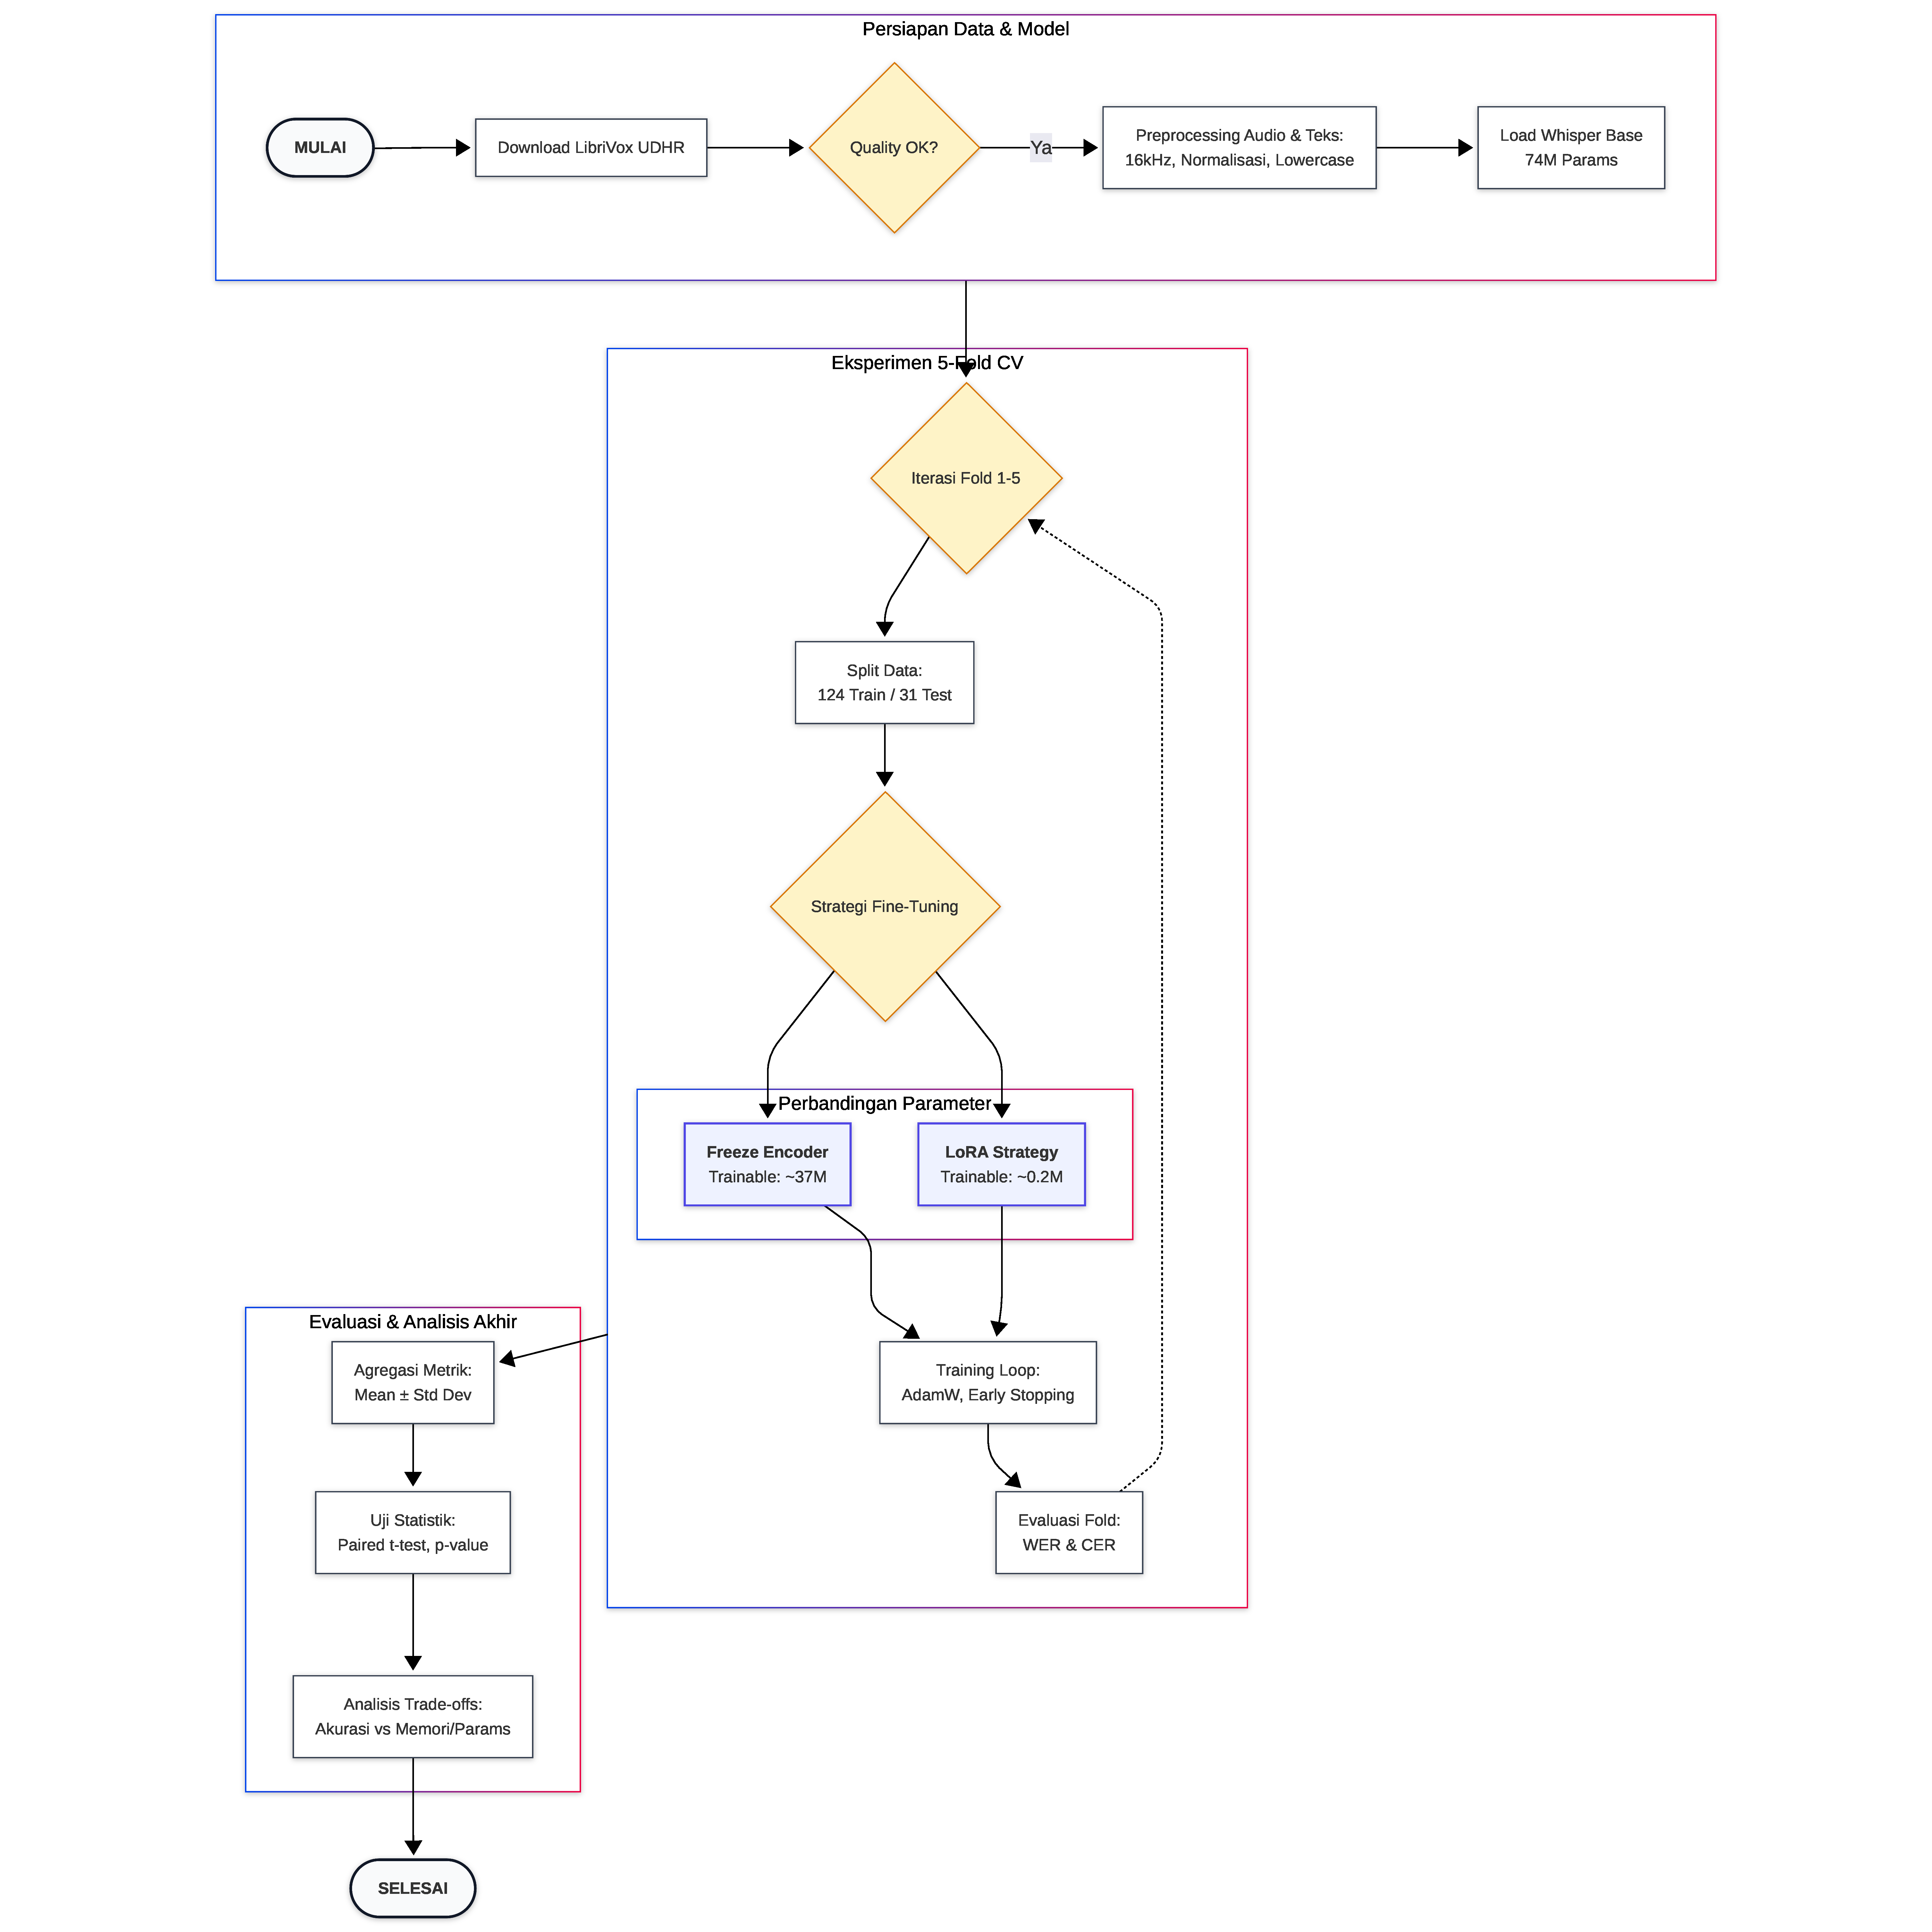
\includegraphics[width=0.8\textwidth]{figure/Development_Flow.pdf}
\caption{Alur Pengembangan Sistem}
\label{fig:3.alur_dev}
\end{figure}

\subsection{Metodologi Fine-Tuning}
\label{III.Metodologi_FT}

Metodologi fine-tuning mengikuti best practices untuk low-resource ASR:

\subsubsection{Full Fine-Tuning Methodology}

\begin{enumerate}[noitemsep]
    \item Initialize dari pre-trained Whisper Small checkpoint
    \item Freeze feature extractor (convolutional layers)
    \item Unfreeze encoder dan decoder Transformer blocks
    \item Training dengan supervised learning pada dataset Minangkabau
    \item Monitoring validation WER untuk early stopping
    \item Save best checkpoint berdasarkan validation performance
\end{enumerate}

\subsubsection{LoRA Fine-Tuning Methodology}

\begin{enumerate}[noitemsep]
    \item Initialize dari pre-trained Whisper Small checkpoint
    \item Freeze seluruh base model parameters
    \item Inject LoRA adapters pada Query dan Value projections
    \item Training hanya LoRA parameters ($\sim$2\% dari total)
    \item Monitoring validation WER untuk early stopping
    \item Merge LoRA weights dengan base model untuk inference
\end{enumerate}

\subsection{Metode Pengujian}
\label{III.Metode_Uji}

Pengujian dilakukan secara sistematis untuk memvalidasi performa model:

\subsubsection{Functional Testing}

\begin{enumerate}[noitemsep]
    \item \textbf{Audio Input Testing}: Verifikasi model dapat menerima berbagai format audio
    \item \textbf{Transcription Testing}: Verifikasi output transkrip dalam format text yang benar
    \item \textbf{Language Identification}: Verifikasi model mengenali bahasa Minangkabau dengan benar
    \item \textbf{Robustness Testing}: Test dengan audio berkualitas rendah, background noise
\end{enumerate}

\subsubsection{Performance Testing}

\begin{enumerate}[noitemsep]
    \item \textbf{Accuracy Testing}: Evaluasi WER dan CER pada test set
    \item \textbf{Inference Speed Testing}: Pengukuran Real-Time Factor (RTF)
    \item \textbf{Memory Usage Testing}: Monitoring GPU/CPU memory consumption
    \item \textbf{Scalability Testing}: Test dengan varying input lengths
\end{enumerate}

\subsubsection{Comparative Testing}

\begin{enumerate}[noitemsep]
    \item Perbandingan Base Whisper Small vs Fine-tuned models
    \item Perbandingan Full Fine-Tuning vs LoRA
    \item Statistical significance testing (paired t-test untuk WER/CER differences)
\end{enumerate}

\section{Ilustrasi Perhitungan Metode}
\label{III.Ilustrasi}

Bagian ini menjelaskan contoh perhitungan untuk metrik evaluasi utama yang digunakan dalam penelitian.

\subsection{Perhitungan Word Error Rate (WER)}
\label{III.Ilustrasi_WER}

WER mengukur edit distance pada level kata antara reference dan hypothesis transcription.

\subsubsection{Formula WER}

\vspace{0.3cm}
\begin{equation}
\label{eq:wer_def}
\text{WER} = \frac{S + D + I}{N} \times 100\%
\end{equation}
\myequations{Definisi WER (Word Error Rate)}
\vspace{0.2cm}

\noindent
di mana:
\begin{itemize}[noitemsep]
    \item $S$ = number of substitutions (kata salah diganti)
    \item $D$ = number of deletions (kata hilang)
    \item $I$ = number of insertions (kata tambahan)
    \item $N$ = total words dalam reference
\end{itemize}

\subsubsection{Contoh Perhitungan}

Misalkan kita memiliki pasangan reference-hypothesis berikut:

\textbf{Reference:} ``\textit{awak ingin pai ka pasar pagi iko}''

\textbf{Hypothesis:} ``\textit{awak ingin pergi pasar pagi ini}''

\textbf{Alignment:}
\begin{table}[H]
\centering
\begin{tabular}{|l|c|c|c|c|c|c|c|}
\hline
\textbf{Reference} & awak & ingin & pai & ka & pasar & pagi & iko \\
\hline
\textbf{Hypothesis} & awak & ingin & pergi & - & pasar & pagi & ini \\
\hline
\textbf{Operation} & C & C & S & D & C & C & S \\
\hline
\end{tabular}
\caption{Alignment untuk perhitungan WER (C=Correct, S=Substitution, D=Deletion)}
\end{table}

\textbf{Perhitungan:}
\begin{itemize}[noitemsep]
    \item Substitutions ($S$): 2 (``pai'' $\rightarrow$ ``pergi'', ``iko'' $\rightarrow$ ``ini'')
    \item Deletions ($D$): 1 (``ka'' dihapus)
    \item Insertions ($I$): 0
    \item Total words ($N$): 7
\end{itemize}

\vspace{0.3cm}
\begin{equation}
\label{eq:wer_example}
\text{WER} = \frac{2 + 1 + 0}{7} \times 100\% = \frac{3}{7} \times 100\% = 42.86\%
\end{equation}
\myequations{Contoh Perhitungan WER}
\vspace{0.2cm}

\subsection{Perhitungan Character Error Rate (CER)}
\label{III.Ilustrasi_CER}

CER mengukur edit distance pada level karakter, lebih sensitif terhadap phonetic errors.

\subsubsection{Formula CER}

\vspace{0.3cm}
\begin{equation}
\label{eq:cer_def}
\text{CER} = \frac{S_c + D_c + I_c}{N_c} \times 100\%
\end{equation}
\myequations{Definisi CER (Character Error Rate)}
\vspace{0.2cm}

\noindent
di mana:
\begin{itemize}[noitemsep]
    \item $S_c$ = number of character substitutions
    \item $D_c$ = number of character deletions
    \item $I_c$ = number of character insertions
    \item $N_c$ = total characters dalam reference
\end{itemize}

\subsubsection{Contoh Perhitungan}

Menggunakan contoh yang sama:

\textbf{Reference:} ``\textit{awakinginpaiakapasarpagiko}'' (tanpa spasi: 30 karakter)

\textbf{Hypothesis:} ``\textit{awakinginpergipasarpagini}'' (tanpa spasi: 28 karakter)

\textbf{Perhitungan:}
\begin{itemize}[noitemsep]
    \item Character substitutions ($S_c$): 5 (``p''→``p'', ``a''→``e'', ``i''→``r'', ``k''→``g'', ``o''→``i'')
    \item Character deletions ($D_c$): 2 (``k'', ``a'' dari kata ``ka'')
    \item Character insertions ($I_c$): 0
    \item Total characters ($N_c$): 30
\end{itemize}

\vspace{0.3cm}
\begin{equation}
\label{eq:cer_example}
\text{CER} = \frac{5 + 2 + 0}{30} \times 100\% = \frac{7}{30} \times 100\% = 23.33\%
\end{equation}
\myequations{Contoh Perhitungan CER}
\vspace{0.2cm}

\noindent
Perhatikan bahwa CER (23.33\%) lebih rendah dari WER (42.86\%) karena partial word matches dihargai pada level karakter.

\subsection{Perhitungan LoRA Parameters}
\label{III.Ilustrasi_LoRA}

Perhitungan jumlah trainable parameters untuk LoRA adaptation.

\subsubsection{Formula LoRA Parameters}

Untuk setiap attention layer dengan projection weight $W \in \mathbb{R}^{d \times k}$, LoRA menambahkan:

\vspace{0.3cm}
\begin{equation}
\label{eq:lora_params}
\text{LoRA params} = r \times (d + k)
\end{equation}
\myequations{Formula Parameter LoRA}
\vspace{0.2cm}

\noindent
di mana $r$ adalah rank.

\subsubsection{Contoh Perhitungan untuk Whisper Small}

Whisper Small memiliki:
\begin{itemize}[noitemsep]
    \item Total layers: 24 (12 encoder + 12 decoder)
    \item Hidden dimension ($d$): 768
    \item Projection dimension ($k$): 768
    \item LoRA rank ($r$): 8
    \item LoRA applied to: Query dan Value projections (2 per layer)
\end{itemize}

\textbf{Perhitungan per layer:}

\vspace{0.3cm}
\begin{equation}
\label{eq:lora_per_projection}
\text{Params per projection} = 8 \times (768 + 768) = 8 \times 1536 = 12,288
\end{equation}
\myequations{Parameter LoRA Per Projection}
\vspace{0.2cm}

\vspace{0.3cm}
\begin{equation}
\label{eq:lora_per_layer}
\text{Params per layer} = 2 \times 12,288 = 24,576
\end{equation}
\myequations{Parameter LoRA Per Layer}
\vspace{0.2cm}

\textbf{Total LoRA parameters:}

\vspace{0.3cm}
\begin{equation}
\label{eq:lora_total}
\text{Total LoRA params} = 24 \times 24,576 = 589,824 \approx 0.59\text{M}
\end{equation}
\myequations{Total Parameter LoRA}
\vspace{0.2cm}

\textbf{Percentage of total parameters:}

\vspace{0.3cm}
\begin{equation}
\label{eq:lora_percentage}
\text{Percentage} = \frac{589,824}{244,000,000} \times 100\% \approx 0.24\%
\end{equation}
\myequations{Persentase Parameter LoRA Terhadap Total}
\vspace{0.2cm}

\noindent
Ini menunjukkan bahwa LoRA hanya melatih $\sim$0.24\% dari total parameters Whisper Small, sangat efisien dibanding full fine-tuning.

